% !TeX root = ../main.tex
\chapter{Related Work}\label{chapter:related-work}


% ModControl – Mobile Phones as a Versatile Interaction Device for Large Screen Applications
%\section{Mobile Phones as a Versatile Interaction Device for Large Screen Applications}\label{section:mobile-phones-interaction-device-large-screen}
\section{Deller et al.}\label{section:deller-2011}
\citeauthor{Deller.2011} propose a modular framework to enable multi-user interactions between smartphones and large-screen applications. A typical client-server architecture with an XML\footnote{XML is a standardized data exchange format, that uses human-readable text.}-based protocol is used. They differentiate between application clients (the large screen) and interaction clients (the smartphones).

The client app is provided with different modules. Some modules offer similar functionality like the experiments implemented in this thesis: The text module enables the user to enter a text; The accelerometer/magnetometer module sends \gls{IMU} data like acceleration and magnetic field data in the background to the server. They also described how they integrated their framework in an application where users can navigate a map and toggle display settings~\cite{Deller.2011}.

The approach presented in this thesis uses a similar architecture. Not only the client-server structure is similar, but also the modularized abstraction is used in so-called \enquote{Interactions}.


% Phone-based motion control in VR (Klinker)
%\section{Phone-based Motion Control in VR}\label{section:phone-based-motion-control-vr}
\section{Benzina et al.}\label{section:benzina-2011}
\citeauthor{Benzina.2011} introduce a system for flying through \glspl{VE} by using a smartphone as input device.
% Since the sight is occluded by the \gls{HMD}, the phone display cannot be used to display information.
They try to find a convenient mappings between the users' actions with the mobile phone and the subsequent reactions in the \gls{VE}. To solve this, they investigate the \glspl{DOF} required to implement a quickly learnable and comfortable travel task.

Different methods using the accelerometer, magnetic field sensor, and touch screen of controlling the flight movement are presented and evaluated. They concluded that the most accurate method for controlling the flight uses an approach, where an airplane metaphor (four \glspl{DOF}) is simulated~\cite{Benzina.2011}.

\citeauthor{Benzina.2011} use the orientational and the touch screen data, the phone provides, to control a \gls{VE}, as is done in this thesis.


% Mobile Devices for Interaction in Immersive Virtual Environments
%\section{Mobile Devices for Interaction in Immersive Virtual Environments}\label{section:mobile-devices-interaction-ve}
\section{Dias et al.}\label{section:dias-2018}
\citeauthor{Dias.2018} propose a solution, where the smartphone has a visual representation in \gls{VR}. The visual representation displays information and a \gls{UI} on its virtual screen. The camera in the smartphone tracks a marker on the \gls{HMD} to track it's own position relativ to the headset. The setup is shown in Figure~\ref{fig:dias-2018}.

\begin{figure}[H]
	\centering
	\begin{subfigure}[t]{0.48\textwidth}%
		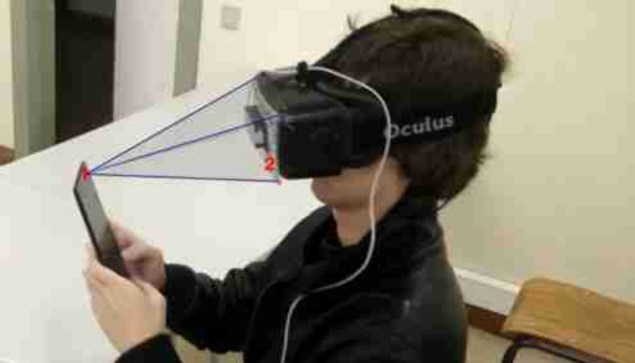
\includegraphics[width=\textwidth]{figures/related_work/dias_2018_tracking.png}
		\caption{The front camera of the smartphone tracks the marker on the \gls{HMD}.}\label{fig:dias-2018-tracking}% chktex 9 % chktex 10
	\end{subfigure}%
	\hspace{0.04\textwidth}%
	\begin{subfigure}[t]{0.48\textwidth}%
		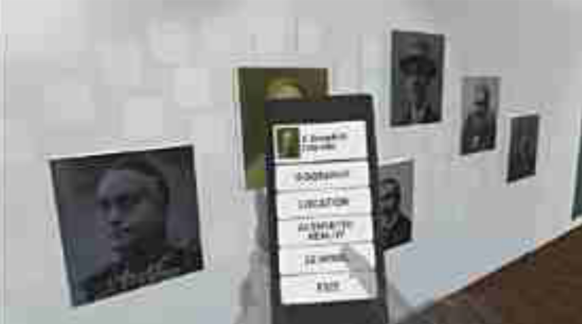
\includegraphics[width=\textwidth]{figures/related_work/dias_2018_virtual_smartphone.png}
		\caption{The virtual smartphone representation and hand avatar in the \gls{VE} while interacting with the \gls{UI}.}\label{fig:dias-2018-virtual-smartphone}
	\end{subfigure}%
	\caption[Tracking setup by Dias et al.]{The tracking system by \citeauthor{Dias.2018}~\protect\cite[4,5]{Dias.2018}.}\label{fig:dias-2018}
\end{figure}

Because the user interacts with the \gls{UI} using the touch screen of the phone as he or she would in real life, the fingers have to be tracked and visualized. Otherwise, the user would not know where his fingers are going to hit the touch screen because the sight is occluded physically by the \gls{HMD}. To solve this problem, they attach a Leap Motion sensor to the \gls{HMD}, which tracks the fingers and displays a hand avatar~\cite{Dias.2018}.

Almost the same research team (\citeauthor{Afonso.2017}) evaluated a selection task using a tablet as an input device in \gls{VR} using the same \gls{VR} setup. They compare the selection time of users selecting a button on the tablet using a realistic hand avatar, a translucent hand avatar, and without any avatar of the hand. Surprisingly, the evaluation shows that users performed the best without any virtual avatar. The authors explain that this is due to the tracking inaccuracies of the tablet and hand. However, users made fewer selection errors when an avatar was displayed~\cite[247-248]{Afonso.2017}.

Those papers are especially useful for the research of this thesis because they introduce a visual representation of the smartphone in \gls{VR} as this thesis uses, too. 


% Design and Implementation of an Immersive Virtual Reality System based on a Smartphone Platform
%\section{Design and Implementation of an Immersive VR System based on a Smartphone Platform}\label{section:design-implementation-vr-system-smartphone-platform}
\section{Steed at al.}\label{section:steed-2013}
The approach by \citeauthor{Steed.2013} also used a smartphone and a \gls{VR} headset as well as a visual representation of the phone. However, since they do not have positional tracking for the smartphone, the position is fixed relative to the position of the \gls{HMD}. There are two different possible positions, one in front of the \gls{HMD} (shown in Figure~\ref{fig:steed-2013-laser-pointer}) and the other one in front of the stomach (shown in Figure~\ref{fig:steed-2013-ui}). The position switches if a hand raise gesture with the phone in the hand is detected. Gestures and orientation of the smartphone are detected using the data of the \gls{IMU}.

\begin{figure}[H]
	\centering
	\begin{subfigure}[t]{0.45\textwidth}%
		\centering%
		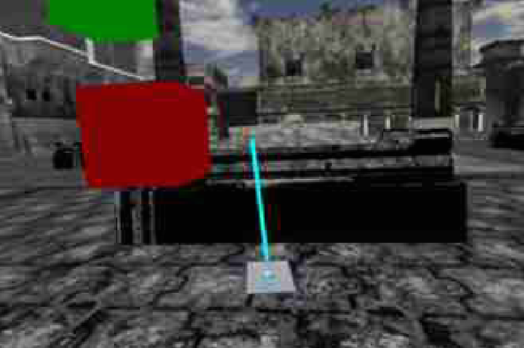
\includegraphics[height=4cm]{figures/related_work/steed_2013_laser_pointer.png}
		\caption{The virtual device in selection mode.}\label{fig:steed-2013-laser-pointer}% chktex 9 % chktex 10
	\end{subfigure}%
	\hspace{0.1\textwidth}%
	\begin{subfigure}[t]{0.45\textwidth}%
		\centering%
		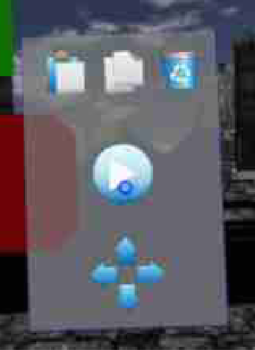
\includegraphics[height=4cm]{figures/related_work/steed_2013_ui.png}
		\caption{The virtual \gls{UI} and the cursor.}\label{fig:steed-2013-ui}
	\end{subfigure}%
	\caption[Virtual smartphone representation by Steep et al.]{The virtual smartphone representation by \citeauthor{Steed.2013}~\protect\cite[43]{Steed.2013}.}\label{fig:steed-2013}
\end{figure}

On the virtual phone screen, a \gls{UI} is displayed as seen in Figure~\ref{fig:steed-2013-ui}. This \gls{UI} has control elements like buttons, which amongst others, can be used to toggle a selection mode. In the selection mode, the phone casts a ray out of the top (similar to a laser pointer) as seen in Figure~\ref{fig:steed-2013-laser-pointer}. The ray direction can be changed by rotating the smartphone. As soon as a \gls{UI}-button is pressed, the objects intersecting with the ray are selected~\cite{Steed.2013}.

A similar laser pointer selection approach is implemented in one of the experiments in this thesis. Also, the selection cursor and the fixed phone position inspired experiments.

